\documentclass[a4paper, 12pt]{article}
\usepackage[T1]{fontenc}
\usepackage[utf8]{inputenc}
\usepackage{apacite}
\usepackage{mathptmx}
\usepackage{enumerate}
\usepackage[margin=0.5in]{geometry}
\usepackage{xspace}
\usepackage{tikz}
\usepackage{parskip} 


% chart attributes
\usetikzlibrary{shapes.geometric, arrows}
\tikzstyle{startstop} = [rectangle, rounded corners, minimum width=5cm, minimum height=1cm, text centered, draw=black, fill=green!30] %start
\tikzstyle{process} = [rectangle, minimum width=5cm, minimum height=1cm, text centered, draw=black, fill=blue!30] %process
\tikzstyle{arrow} = [thick,->,>=stealth] %arrow for chart

\renewcommand{\baselinestretch}{1.0}

\newcommand\nd{\textsuperscript{nd}\xspace}
\newcommand\rd{\textsuperscript{rd}\xspace}
\newcommand\nth{\textsuperscript{th}\xspace} %\th is taken already

\setlength\parindent{0pt} % set paragraph indent to zero

% fill up your name, ID, contribution and paper title here
\author{
LOA TAT ANN \quad 1221304731 \quad contribution1 \\
YU BUI XUAN \quad 241UC24121 \quad contribution2\\
MOHD SYAMEL BIN MOHD KARID \quad 1221309130 \quad contribution3\\
}
\title{ Optimizing DDoS Attack Detection with Machine Learning Algorithms and Multiple Datasets }

\begin{document}
\maketitle

%dataset size
%impact of datasets affecting the accuracy of machine learning DDoS detection methods (?)

\section*{Executive Summary}
%This includes the problem statement, objectives, research methodology, expected output and significance of output in a summary form. 

Distributed Denial-of-Service (DDoS) attacks have caused massive disruptions to network services, and they are difficult to detect as they blend in within normal traffic to evade detectors. Researchers have developed new methods, such as machine learning, to prevent threats from happening. Researchers prize machine learning for its excellent performance, but one of its key limitations is a lack of suitable datasets and algorithms. The study aims to address dataset inadequacies and algorithm performance, which are some of the key challenges faced by researchers. Existing approaches used by researchers often get inaccurate results, as most of them use outdated datasets or datasets with questionable quality. Besides that, each algorithm has its strengths and weaknesses. This study will assess the effectiveness of various techniques under diverse conditions by employing multiple datasets and a blend of ensemble methods to determine which methods are the most optimal for different tasks. Several phases including data processing, extraction of information, classification and evaluation are conducted as a basis for the research. After that, a solution is developed based on the findings, and it will endure a thorough testing procedure to prove the legitimacy of findings. The findings of this research will be significant - organizations can implement practical solutions and researchers can advance machine learning and cybersecurity.

\textbf{Keywords:} \textit{research, cybersecurity, artificial intelligence, machine learning, ddos, ddos attacks, algorithms, dataset, optimization, ensemble}

\section{Introduction}
%This section contains a brief introduction to the research topic and background. \\
%Citation example: \citeA{1}

Distributed Denial-of-Service (DDoS) is a cyberattack method that utilizes multiple benign devices on a network and uses them to send malicious packets to disrupt networks with hopes of denying others normal access to them. DDoS attacks are difficult to detect, as they blend in with normal network traffic and use illegitimately obtained IP addresses to avoid being detected. \citeA{1} Because of this, it is hard to detect DDoS attacks which can cause massive damage to network infrastructure. Due to the increasing popularity of network technology, DDoS attacks are becoming more commonplace. According to a report from Cisco, they estimated recording around 15.4 million DDoS attacks. \citeA{10} 

With the threats of such attacks, researchers develop various methods to detect DDoS attacks and prevent them from happening. The method proposed by researchers is machine learning detection, as they prize its performance and adaptability on such tasks. However, machine learning methods still face issues, including the fact that the varying quality and quantity of datasets and algorithms can lead to varied results. These datasets and algorithms are crucial to machine learning as they serve as a “guideline” to help the algorithms detect threats more accurately. As DDoS attacks develop rapidly, current methods may not be capable of reacting to these new threats. \citeA{1}

In this research proposal, we will explore the methods to create a solution that optimizes machine learning on DDoS attack detection with the use of multiple algorithms and datasets. The research will comprehensively evaluate, compare and determine the best methods in a period spanning several years of research and development. We will also propose the related activities in research and get the expected results from there.

\section{Problem Statement}
We have identified that dataset and algorithm issues are some of the major reasons for inaccuracies in attack detection among machine learning. The dataset is a major part of machine learning detection, as it uses the dataset to extract meaningful information to compare and detect similarities. Besides that, machine learning algorithms require the correct datasets to detect and treat the attack properly. \citeA{2} 

Studies have also stated that the lack of associated datasets and their features useful for cross-comparison is a major limitation of current research on machine learning in DDoS attack detection. \citeA{1}  Also, not all datasets are comparable to each other, leading to data discrepancies. Besides that, most datasets used are outdated, redundant or contain insufficient information. For instance, the CICDDoS2019 dataset only contains 1\% of benign records, with most records being hostile, leading to an imbalance of data and bias in classification. \citeA{1} This could cause difficulty for machine learning algorithms in detecting traffic and accidentally classifying benign traffic as a threat to the network, affecting real-time deployment.

Researchers have proposed different methods to detect DDoS attacks, and there are differences in algorithms in various methods employed by the algorithms. Some methods, such as Support Vector Machines (SVM) and Random Forest, have excellent performance in detection, while others have recorded weaker results. Researchers use different setups for their methods to conduct experiments which contributed to the difference in test results. \citeA{8} Application of such methods also varies depending on the algorithm, where some algorithms are harder to implement than others because of a complex structure. \cite{9} 

\clearpage

\section{Research Questions, Hypotheses and Objectives}
%Minimum of two and maximum of four for each of the research questions, hypotheses, and research objectives. You can use numbering/bullet point to list them out.

\subsection{Research Questions}
\begin{enumerate}
  \item How does dataset quality affect the accuracy of machine learning algorithms in DDoS attack detection?
  \item How do ensemble methods, which combine multiple machine learning algorithms, compare to individual algorithms in terms of accuracy and robustness for DDoS attack detection?
\end{enumerate}

\subsection{Hypotheses}
\begin{enumerate}
  \item The quality of datasets, which include the completeness and relevance of data, could significantly affect the accuracy of detecting DDoS attacks in IoT environments.
  \item Ensemble methods that combine multiple machine learning algorithms offer higher accuracy and robustness in DDoS attack detection compared with single algorithms.
\end{enumerate}

\subsection{Objectives}
\begin{enumerate}
  \item To evaluate the impact of dataset quality in the aspect of data completeness and relevance on the accuracy of DDoS attack detection.
  \item To prove the performance of ensemble methods is better than individual machine learning algorithms in terms of accuracy and robustness for DDoS attack detection. 
\end{enumerate}

\section{Literature Review Summary}

In the papers of \citeA{6}, they approach DDoS detection with methods like Random Forests and SVMs that demonstrate high accuracy in their tests. However, their effectiveness is determined by the dataset's relevance and completeness. Using a poor-quality dataset can lead to an increasing number of false positives which could affect the reliability of these models.

Researchers show another issue involving datasets in the research \citeA{5} states that the Bidirectional long short-term memory (BiLSTM) method performs exceptionally well with an accuracy of 82.8\%, scoring the highest compared to other research methods. However, it could come with the risk of overfitting. This occurs when researchers excessively train the model using the NSL-KDD dataset, which can lead to difficulties. Moreover, the NSL-KDD dataset may not provide an accurate depiction of the network traffic behaviour, potentially impacting the model’s efficacy, particularly in real-life scenarios.

 Next, the use of an ensemble algorithm which is used in GRU-LM  and Word2vec architecture system as researched by \citeA{6}, shows that the accuracy greatly improved compared to when using a single algorithm, as a result shows that the integration of Word2vec and GRU-LM together could achieve the accuracy of 87.83\%, showcasing that the method achieved approximately 30\% higher than other types of models including RNN and LSTM (Long Short-Term Memory). \citeA{6}

\clearpage

\section{Research Methodology}
%This section contains a description of the steps involved in research methodology, which also includes the metrics to be used for evaluating the proposed method along with a brief description of the techniques/models/methods/algorithms to be used.

\subsection{Overview}
The research methodology for the work is divided into stages, which include: pre-processing, data analysis utilizing methods like traffic segmentation and data classification, evaluation and comparison of findings, and the selection and training of algorithms and datasets. Using these research methodologies will assist us in identifying the ideal set of datasets and algorithms for DDoS intrusion detection.

%You can use table/figure/image/graph in the report. All figures must have titles.

\subsection{ Selection and Training of Algorithms with Datasets}

To evaluate the performance a set of machine learning algorithms are selected for the training designed to assess the performance of different methods in detecting DDoS attacks. Several algorithmic approaches are chosen, which include K-Nearest Neighbors (KNN), Support Vector Machines (SVM), Naive Based Classifiers, Random Forest, and others to create an ensemble of algorithms for research. Multiple relevant datasets, such as CCIDS2017, serve as the data sources for the algorithms. \citeA{8}

The training process of such algorithms is split into training and testing subsets, and each of the tests is recorded to extract important features such as packet size and traffic volume. The data are then compared with several metrics. The algorithms are compared by metrics such as accuracy, precision, and recall to determine which algorithm performed best on different conditions, and select the most effective algorithm from there.

\subsection{ Data Preprocessing Techniques }

Data obtained from the datasets must be pre-processed before use. This is done to guarantee that the produced dataset is of sufficient quality and consistently processed to fulfil the input standards of the desired model. To start, data cleansing eliminates entries that can be incomplete and cause biases while training the model. One-hot encoding converts categorical variables without numerical values into bit vectors, the most appropriate format for machine learning models. \citeA{8} Normalization methods like Z-score normalization and Min-Max scaling are then carried out. These techniques are useful in standardizing the appearance of the data and ensuring that features are scaled similarly to improve the model's training process and prevent big numbers from impacting it.

\subsection{ Traffic Segmentation and Feature Extraction }

Traffic segmentation and feature extraction are the key elements in detecting DDoS attacks by discriminating between malicious and normal network traffic. In traffic segmentation, network traffic is split into several segments to make detection tasks easier. Methods such as Gaussian filtering are also employed to reduce the noise of recorded data and help identify important information for network traffic. \citeA{9} Then, important features are extracted with several techniques such as Principal Component Analysis to identify significant features for classification. The finalized data could be used to augment the database extending its accuracy and capacity.

\subsection{ Classification Approach with Neural Networks }

The classification phase utilizes neural networks, specifically LSTM networks, recognized for their capacity to preserve information over sequences, rendering them appropriate for the analysis of time-series data which will be utilized in research\cite {2}. These networks are trained with the selected features from the segmentation phase. Advanced optimizing algorithms like Adam (Adaptive Moment Estimation) are used to optimize the model weights iteratively, ensuring faster convergence during training. \citeA{2} This step allows the model to learn complex relationships within the data, resulting in more accurate classification outcomes.

\subsection{ Model Evaluation Metrics }

For the performance examination of the proposed models, the following measures will be employed, accuracy, precision, recall and F1 score. Accuracy calculates the ratio of total instances that are predicted to be in one category out of total cases, and precision quantifies how many of the total instances identified to be in one specific category are actually in that category. Recall checks how well the model ‘catches’ all cases related to the category. The F1 score has the best characteristics when calculating the ratio between the number of true positives and both true and false positives and is highly suitable when working with imbalanced datasets \citeA{8}. They provide a full-scale assessment, and it is safe to assume that the chosen model is precise and consistent in identifying anomalies.

\subsection{ Comparative Analysis of Classifiers }

This study explores many other classifiers gathered from tests such as Support Vector Machines (SVM), K-Nearest Neighbors (KNN), Random Forest, and Logistic Regression compared with neural networks \citeA{8}. Every algorithm is then compared in terms of certain criteria they provide, including accuracy, precision, recall and required computational time. This comparative analysis will help to define what pros and cons of each model exist, which in turn makes it easy to choose the proper algorithm for the task. The hope of achieving this is through comparing these models to the neural networks; thus, the kind of approach chosen meets the requisite efficiency and reliability in the classification of abnormalities in detecting DDoS attacks.

This research approach guarantees the thorough and strategic approach of data pre-processing, feature selection/extraction, model training and testing processes by enhancing the robustness of the solution.

\subsection { Development, Testing and Reporting }

After the previous sections are fully processed and selected, a demonstration system will be created using known network and computing technologies. The finished system will be first tested in a controlled network environment, and after that, it will be deployed in real-world environments for a much more realistic look at its performance. An error-checking session will be conducted should the system detect anomalies, and it will be addressed properly. After the testing, a final evaluation will be conducted before reports are made and published. 

\clearpage

\section{Research Activities and Milestones}

\subsection{Flowchart for Activities}

Figure \ref{graph:1} is a flow chart showing the procedures involved in the research. 
%Flowchart
\begin{figure}[ht]
    \centering
    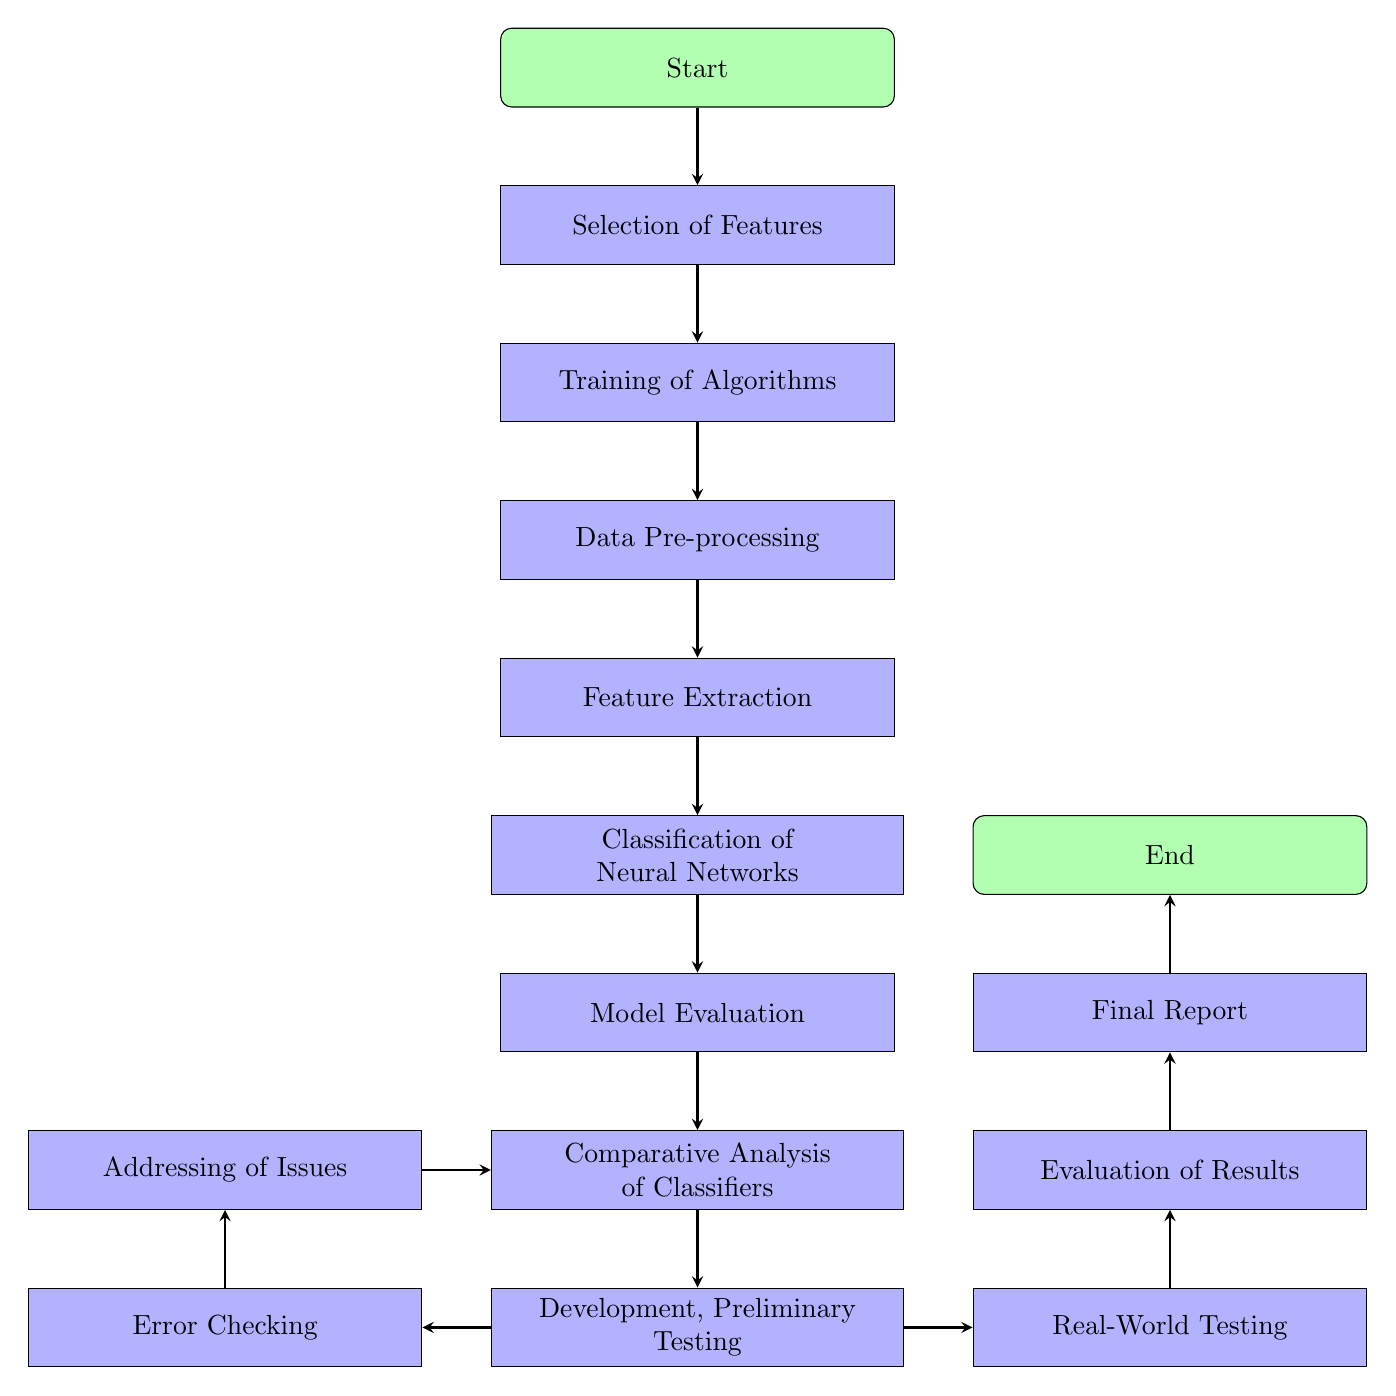
\begin{tikzpicture}[node distance=2cm]
    %nodes
    \node (start) [startstop] {Start};
    \node (proc) [process, below of=start] {Selection of Features};
    \node (proc1) [process, below of=proc] {Training of Algorithms};
    \node (proc2) [process, below of=proc1] {Data Pre-processing};
    \node (proc3) [process, below of=proc2] {Feature Extraction};
    \node (proc4) [process, below of=proc3] {\parbox{5cm}{\centering Classification of\\Neural Networks}};
    \node (proc5) [process, below of=proc4] {Model Evaluation};
    \node (proc6) [process, below of=proc5] {\parbox{5cm}{\centering Comparative Analysis\\of Classifiers}};
    \node (proc7) [process, below of=proc6] {\parbox{5cm}{\centering Development, Preliminary Testing}};
    \node (proc7a) [process, left of=proc7, xshift=-4cm] { Error Checking };
    \node (proc7b) [process, above of=proc7a] { Addressing of Issues };
    \node (proc8) [process, right of=proc7, xshift=4cm] {Real-World Testing};
    \node (proc9) [process, above of=proc8] {Evaluation of Results};
    \node (proc10) [process, above of=proc9] {Final Report};
    \node (stop) [startstop, above of=proc10] {End};

    %arrows
    \draw [arrow] (start) -- (proc);
    \draw [arrow] (proc) -- (proc1);
    \draw [arrow] (proc1) -- (proc2);
    \draw [arrow] (proc2) -- (proc3);
    \draw [arrow] (proc3) -- (proc4);
    \draw [arrow] (proc4) -- (proc5);
    \draw [arrow] (proc5) -- (proc6);
    \draw [arrow] (proc6) -- (proc7);

    \draw [arrow] (proc7) -- (proc7a);
    \draw [arrow] (proc7a) -- (proc7b);
    \draw [arrow] (proc7b) -- (proc6);

    \draw [arrow] (proc7) -- (proc8);
    \draw [arrow] (proc8) -- (proc9);
    \draw [arrow] (proc9) -- (proc10);
    \draw [arrow] (proc10) -- (stop);
    
    \end{tikzpicture}
    \caption{Flow chart for the research.}
    \label{graph:1}
\end{figure}

\clearpage

\subsection{Activities Gantt Chart}
Figure \ref{gantt:1} and Table \ref{table:1} is a Gantt chart showing how long the research will be conducted and the time details about the research methods.

\begin{figure}[!ht]
    \centering
    \includegraphics[width=1\linewidth]{gantt.png}
    \caption{Gantt Chart}
    \label{gantt:1}
\end{figure}

\begin{table}[!ht]
    \centering
    \begin{tabular}{|l|c|c|c|}
    \hline
        \textbf{Name} & \textbf{Start} & \textbf{Finish} & \textbf{Duration} \\ \hline
        \textbf{Research Proposal} & 2024-09-05 & 2024-09-18 & 14 days \\ \hline
        \textbf{Selection of Features } & 2024-09-18 & 2024-10-15 & 28 days \\ \hline
        \textbf{Training of Algorithm} & 2024-10-14 & 2024-12-08 & 56 days \\ \hline
        \textbf{Data Pre-processing} & 2024-12-08 & 2025-01-11 & 35 days \\ \hline
        \textbf{Feature Extraction} & 2025-01-11 & 2025-01-31 & 21 days \\ \hline
        \textbf{Classification} & 2025-01-31 & 2025-02-27 & 28 days \\ \hline
        \textbf{Model Evaluation and Analysis} & 2025-02-27 & 2025-03-19 & 21 days \\ \hline
        \textbf{Development and Preliminary Testing} & 2025-03-19 & 2025-05-20 & 63 days \\ \hline
        \textbf{Error Checking} & 2025-04-25 & 2025-06-19 & 56 days \\ \hline
        \textbf{Resolve Issues} & 2025-06-05 & 2025-07-30 & 56 days \\ \hline
        \textbf{Real World Testing} & 2025-05-29 & 2025-07-30 & 63 days \\ \hline
        \textbf{Results Evaluation} & 2025-07-30 & 2025-08-19 & 21 days \\ \hline
        \textbf{Final Report} & 2025-08-10 & 2025-09-13 & 35 days \\ \hline
    \end{tabular}
    \caption{Table of tasks involved}
    \label{table:1}
\end{table}

\clearpage

\section{Expected Results and Impact}

\subsection{Expected Results}
The main expected result of this research is the improvements in detection performance by selecting the best from multiple datasets and detection algorithms with a testing process. Besides that, we would also compare various algorithms to show other aspects of each algorithm and determine the best from them. By combining the data gathered we can optimize each setup for the most suitable task, enabling higher performance in DDoS attack detection. 

The results from the proposal could also be affected by real-time analysis of network traffic by gathering the results among multiple algorithms. It will also demonstrate its adaptability to various environments and tests can be scaled accordingly to counter various threats. 

\subsection{Expected Impact of Research}

\subsubsection{ Framework for Enhanced Cybersecurity Practices and Methods }

The proposed results can be part of an improved framework designed for real-time DDoS detection and prevention. Organizations can implement the framework in their network systems to improve their security. Implementing the system will lead to better adaptability against novel threats, improved operational stability, increased trust from customers and stakeholders, and compliance with national and state laws. 

\subsubsection{ Industry Adoption and Market Innovation }

Firms can adopt the methods and implement them in various practical applications. Such applications may include real-time network monitoring systems, customized detection frameworks and cyber threat intelligence platforms. The methods can also implemented within existing security systems to improve detection performance. With these implementations, innovators can drive innovation by advancing the field with new creations and ideas.

\subsubsection{ Foundation for Further Improvements and New Discoveries on the Field }

The resulting published work may also contribute to research efforts. The results may be published by reputable journals in the field, which could be used as a guideline for future research, enabling further improvements and new additions to improve the research quality of other journals. It can also be used as a baseline for research in other novel techniques and further advancements in machine learning and cybersecurity further down the line.

\clearpage

%References
\bibliographystyle{apacite}
\bibliography{MyBib}{}


\end{document}

